\section{Software Testing}
\subsection{Types of Tasting}
\paragraph{}Testing is an important part of software development life cycle.  It is performed to ensure quality of the developed system.  Testing includes a set of investigative activities that can be planned in advance and conducted systematically, to assure the stakeholder that system fulfils all the requirements gathered during requirement gathering phase.  Software testing is one of the key elements in software projects that is often referred to as verification and validation.  Verification refers to the set of activities that ensure that software correctly implements specified functionality. Validation refers to a set of activities built around traceability matrix which ensure that the functionality implemented by the system is traceable to customer requirements.

\paragraph{}The software test plan (STP) is designed to test each module to measure its performance, to uncover bugs in the system, to set aright any flaws in logic that may be present, and to check logical flow from one module to another within system.

\subsection{Test cases and Test Results}
\paragraph{}A strategy outlines what to plan, and how to plan it. A successful strategy is your guide through
change, and provides a firm foundation for ongoing improvement. Unlike a plan, which is obsolete
from the point of creation, a strategy reflects the values of an organization - and remains current
and useful. When an organization tests its products or its tools, it tries to compare them against
its expectations and values. By its nature, testing introduces change as problems are identified and
resolved. A test strategy is necessary to allow these two impulses to work together. Furthermore,
testing can never be said to be `complete’, and a core skill in testing is the justified management
of conflicting demands; without a strategy, these judgements will be inconsistent to the point of
failure.
\paragraph{}Software development is a creative process. A test strategy is a vital enabler to this process keeping focus on core values and consistent decision-making to help achieve desired goals with best use of resource. A good strategy stands as a clear counter to reactive, counter-productive test approaches.
\begin{figure}[!h]
	\centering
	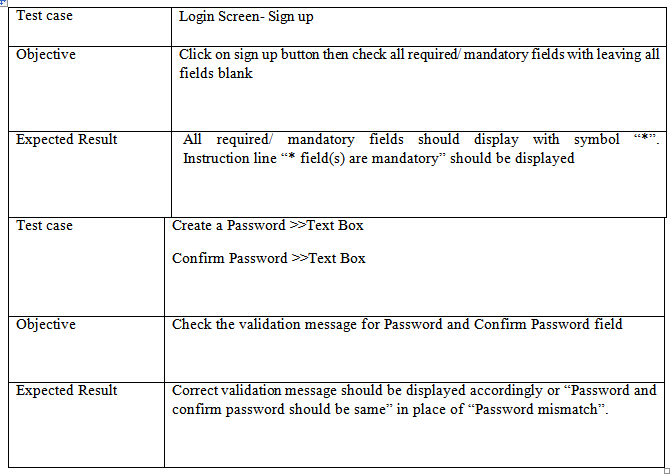
\includegraphics[width = \textwidth]{./testc}
	
\end{figure}
\begin{figure}[!h]
	\centering
	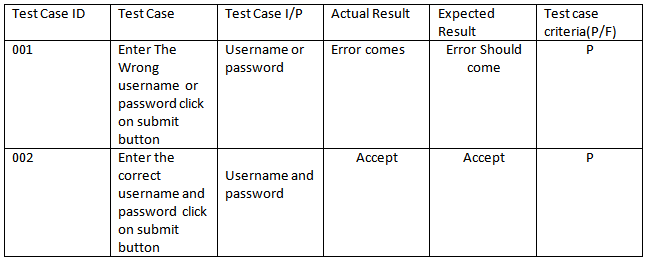
\includegraphics[width = \textwidth]{./testc1}
	
\end{figure}
\begin{figure}[!h]
	\centering
	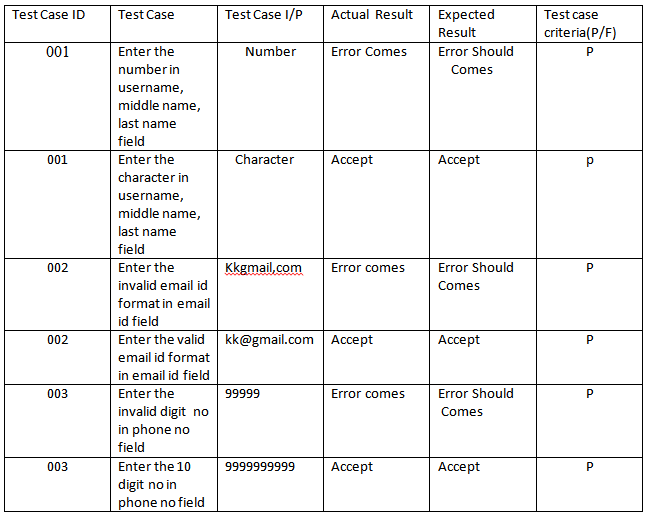
\includegraphics[width = \textwidth]{./testc2}
	
\end{figure}
